\chapter{Setup}

Dieses Kapitel behandelt die Installation und Ersteinrichtung der Suchmaschine über Docker. Die Installation erfolgt dabei über Docker mithilfe von Docker-Compose. Es werden 2 ElasticSearch Instanzen, eine Kibana Instanz und eine Logstash-Instanz aufgesetzt. !!GRAFIK!!

\section{Docker}

Docker ist eine Software zur Virtualiserung von Anwendungen. Dabei wird allerdings nicht wie bei virtuellen Maschinen die gesamte Hardware simuliert, sondern sie laufen im Kontext der Host-Betriebstystems.

Docker-Compose ist ein Tool, mit welchen es erleichtert wird mehrere Docker-Container zu verwalten. Dafür werden in einer YAML-Datei die gewünschten Docker Container eingetragen \ref{lst:es01}. Dabei können Einstellungen wie der Container-Name Docker-Compose liest nun diese Datei und erstellt damit die Container und Netzwerke alle automatisch.

\subsection{Rechteverwaltung in Docker}

Ein kurzer Exkurs zur Rechteverwaltung in Docker. Will ein Docker-Container aus das Host System schreiben, so nutzt dieser die Berechtigungen des Users innerhalb des Docker-Containers. Nun kann es allerdings passieren, das die Nutzer-ID des Docker-Containers nicht der Nutzer-ID des Hosts entspricht. Legt man nun Dateien im Hostsystem ab, welche vom Container gelesen werden, muss dabei auch die Rechte geachtet werden. 

ElasticSearch verwendet die UID und GUID von 1000. Auf dem Host System ist dies jedoch ein komplett anderer Nutzer. Das kann zu Problemen führen, da nun Dateien, welche für ElasticSearch gedacht sind einen Nutzer, welcher nicht zu diesem Projekt gehört, gehören. Der Nutzer wurde nun auf eine andere UID gesetzt, um Verwirrung zu vermeiden. \cite{JarrodWeaver.2014}

\section{ElasticSearch}

Die beiden ElasticSearch Instanzen bilden das Kernstück dieses Setups. Sie werden die Daten verwalten und sich untereinander synchronisieren. Dafür werden die beiden Instanzen geclustert.

\begin{lstlisting}[language=XML, frame=single, label={lst:es01}] 
	es01:
	image: docker.elastic.co/elasticsearch/elasticsearch:7.5.1
	container_name: es01
	environment:
		- "ES_JAVA_OPTS=-Xms4g -Xmx4g"
	ulimits:
		memlock: -1
	volumes:
		- /srv/elk/elasticSearch01/:/usr/share/elasticsearch/data
		- /srv/elk/config/elasticsearch.yml:
			/usr/share/elasticsearch/config/elasticsearch.yml
	ports:
		- 9200:9200
	networks:
		- elastic
\end{lstlisting}

In diesem Auschnitt aus der Docker-Compose werden nun die ersten grundlegenden Einstellungen getroffen.

Für die beiden ElasticSearch Instanzen wir der Java-Speicher auf 4 Gigabyte gesetzt. Dies errechnet sich dadurch, dass der Server 16 Gigabyte RAM besitzt und die ElasticSearch Instanzen niemals mehr als 50 \% des gesamten RAMs verwenden sollten. \cite{ElasticsearchB.V..12172019}

Der ulimits Befehl hebt die Begrenzung des Memory-Locks auf, damit ElasticSearch korrekt arbeiten kann. Dadurch wird der RAM von ElasticSearch nicht in den SWAP-Speicher gelegt. Dies würde die Leistung von der Suchmaschine stark beinträchtigen.

Als Volumes ist zum einen die oben genannte YAML-Datei angegeben und zum anderen wird der Datenordner gemountet. Dies dient dazu, dass, falls der Container zerstört wird, die indexierten Daten trotzdem weiterhin gespeichert werden.

Der Port wird zum Host-System durchgereicht, damit das System auch von außerhalb des Docker-Netwerkes zu erreichen ist. Dabei ist das System trotz blockierter UFW zu erreichen. Dies liegt daran, dass die Docker-Container in der Standardeinstellung die UFW ignorieren.

In der ElasticSearch-Konfigurationsdatei werden nun die Einstellungen, die speziell für das ElasticSearch-System relevant sind verwaltet \ref{lst:es01-yml}. 

\begin{lstlisting}[language=XML, frame=single, label={lst:es01-yml}] 
	cluster.name: dietrich-online-cluster
	node.name: es01
	bootstrap.memory_lock: true
	network.host: 0.0.0.0
	discovery.seed_hosts: ["es02"]
	cluster.initial_master_nodes: ["es01", "es02"]
\end{lstlisting}

Darin wird zuerst der Cluster-Name definiert. Dieser dient dazu, dass die Server wissen, dass Sie dieselben Daten betreuen. 
Danach wird der Name des Servers vergeben. Dieser wird für spätere Einstellungen noch wichtig.

Das Memory-Lock Setting dient dazu, dass die Anwendung verhindert, dass sie in den SWAP gelegt wird.

Der Network Host wird hier auf alle Interfaces der Maschine gesetzt, damit sich alle System innerhalb der Docker Netzwerkes finden können.
Das Seed-Host Setting sagt aus, an welche Nodes die Daten synchronisiert werden sollen.

Der letzte Eintrag dient dazu, dass bei der ersten Synchronisation das System weiß, welche Nodes alle Daten enthalten, also mit welchen Server sich synchronisiert werden soll. Da hier beide Systeme beim ersten Start noch keine Daten besitzen, sind alle Nodes zu beginnt Master. 


\section{Kibana}

Die Grundkonfiguration von Kibana ist einfacherer als die Konfiguration von ElasticSearch. Es muss nur die YAML-Datei gemountet werden und der Port 5601 nach außen durchgereicht werden.

In der Konigurationsdatei werden nun die Einstellungen für Kibana gesetzt. Darunter fällt der oben genannte Port, der Server-Host, in diesem Fall auch 0.0.0.0, und die ElasticSearch-Hosts. Dabei werden alle Server Instanzen mitgegeben, auf denen Kibana arbeiten soll. 

\section{Logstash}

Für die Grundkonfiguration von Logstash muss, wie schon im Ersteindruck, der Treiber in die Core-Bibliothek gelegt werden. Zudem werden die Konfigurationsdateien für die Pipelines, also die Prozesse des Daten sammeln und an ElasticSearch gemountet.

In der Konfigurationsdatei für Logstash wird dann der Name, die Pipeline.id und die Pipeline-Worker festgelegt. Die Pipeline-Worker sind die Threads in denen eine der konfigurierten Pipelines abgearbeitet wird. Generell sollte die Anzahl der Cores auch die maximale Anzahl der Worker sein.


\section{X-Security}

X-Security nennt sich das Paket mit den Sicherheitseinstellungen für den ELK-Stack. In diesem Schritt  wird hier den kompletten Traffic zwischen den einzelnen Komponenten, sowie der Endnutzer zum Server mit SSL verschlüsselt. 

Dazu mussten zuerst einmal die Zertifikate generiert werden. Dafür bietet ElasticSearch ein Tool an, welches eine Zertifikats-Autorität\footnote{Mithilfe einer CA kann sich ein Klient gegenüber des Servers ausweisen und umgekehrt.} (CA) und die einzelnen Zertifikate mit Private und Public-Key generiert. Allerdings werden diese standardmäßig im PKCS 12-Format abgespeichert. Dieses ist ein Container-Format, welches die Schlüssel und die CA zusammen verpackt. Jedoch benötigt Kibana zum Beispiel nur die Autorität als einzelnes Zertifikat und nicht in einem Container.

Normalerweise gibt es eine Möglichkeit dieses Zertifikat aus der PK12-Datei zu entpacken, jedoch gab es hierbei Probleme, da OpenSSL, das Tool welches zum Entpacken verwendet wird, die CA nicht richtig entpacken kann. \cite{nerophon.2018}

Die Lösung dieses Problems war es schon bei der Zertifikat-Erstellung eine Option mitzugeben, dass die Zertifikate nicht verpackt werden sollen. 

Um nun alle Zertifikate gleichzeitig zu generieren, kann eine YAML Datei mitgegeben werden. In dieser werden dann die Details für die Zertifikate wie zum Beispiel DNS-Name und IP des Servers mitgegeben werden. In diesem Fall wurde nur der DNS-Name angegeben \ref{lst:certs-yml}.

\begin{lstlisting}[language=XML, frame=single, label={lst:certs-yml}] 
	instances:
	- name: 'es01'
	  dns: [ 'es01', 'bib55', 'bib55.uni-trier.de' ]
	  [...]
\end{lstlisting}

Damit diese Zertifikate auch genutzt werden können musste nun jeder Container das zugehörige Zertifikat mounten. Zudem wurde in den dazugehörigen Konfigrationsdateien die jeweiligen Optionen zur Nutzung der CA und Private Keys gesetzt werden.

Zusätzlich zu den Zertifikaten muss auch noch eine Password Authentifikation eingebaut werden. Dazu kann auf den ElasticSearch-Containern ein Befehl zur Erstellung der Systempasswörter aufgerufen werden. Dadurch werden alle Benuzter, welche die einzelene Systeme wie Logstash oder Kibana zum funktionieren brauchen generiert.

Auch diese müssen in den Konfigrationsdateien vermerkt werden. Weitere Nutzer können von nun an per API oder Kibana erstellt werden. Die Verteilung der Rechte passiert hierbei rollen-basiert. Es wird zuerst eine Rolle erstellt, welche die gewünschten Rechte enthält, welche daraufhin an den Nutzer weitergegeben wird. Dabei können die Rollen sehr spezifisch angepasst werden. Es können einzelen Systemfunktionen wie die zum Beispiel die Erstellung von Snapshots spezifisch freigegeben werden. Hierbei sollte sich an das minimal Prinzip gehalten werden, also nur so viele Rechte vergeben, wie der Nutzer definitiv benötigt.

Um nun einen Query gegen das ElasticSearch System zu stellen, muss zum einen eine BasicAuth sowie das CA mitgegeben werden \ref{lst:curlQuery}.

\begin{lstlisting}[language=BASH, frame=single, label={lst:curlQuery}] 
	curl https://bib55:9200 --cacert ca.crt -uuser:pass
\end{lstlisting}

Damit nun auch Logstash wieder Daten an ElasticSearch senden kann, wird ein Nutzer erstellt, welcher nur auf Indices mit mit dem Präfix dietrich\_ Zugriff erhält. Die Erstellung dieses Nutzer wurde dabei die Benuzter-Oberfläche von Kibana gemacht \ref{img:kibanaRoles}. 

\begin{figure}
	\centering
	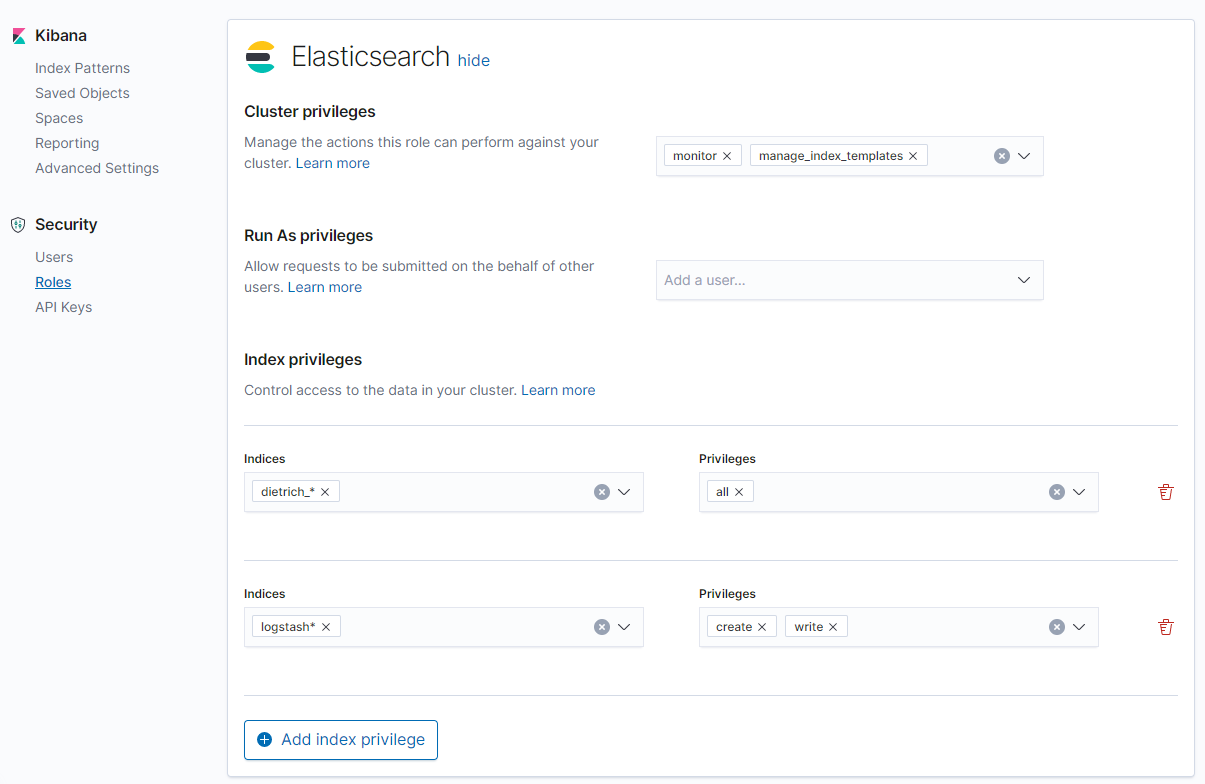
\includegraphics[width=1\linewidth]{images/setup/kibana_roles.png}
	\caption{Seite zu Erstellung von Rechte-Rollen}
	\label{img:kibanaRoles}
\end{figure}